\documentclass[UEF8]{ctexart}
\usepackage{fontspec}
\setmainfont[Mapping=tex-text]{Noto Sans CJK TC Thin}
\usepackage[utf8]{inputenc}
\usepackage{indentfirst}
\usepackage{amsmath}
\usepackage{ctex}
\usepackage{amsfonts}
\usepackage{amssymb}
\usepackage{listings}
\usepackage{graphicx}
\usepackage{gensymb}
\usepackage{multicol}
\usepackage[width=16.00cm, height=24.00cm]{geometry}
\usepackage{geometry}
%\setCJKmainfont[BoldFont=SimHei]{SimSun}
%\setCJKmonofont{SimSun}     
\parindent 2em 
\setlength{\columnseprule}{1pt}
\setlength\columnsep{1cm}

\title{弗兰克-赫兹实验报告}
\author{余丰\quad PB19000261}
\date{2020/11/26}


\begin{document}
\maketitle

{\bfseries 摘要} \quad 本次实验使用微机型弗兰克-赫兹实验仪测定了氩原子来证明原子能级存在以及进一步了解波尔原子论。

\begin{multicols}{2}
\section{实验简介}
\subsection{实验原理}
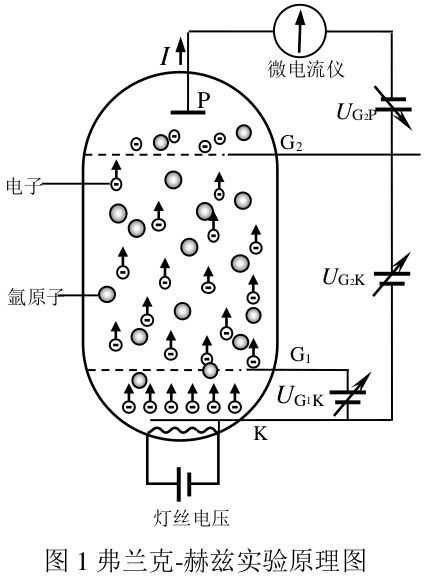
\includegraphics[scale=0.42]{p1.png}

 如图1所示,电子在K-$G_{1}$区间被电场加速,随后在$G_{1}$-$G_{2}$区间继续加速并与氩原子相撞,当电子动能超过第一激发态与基态的能级差$\Delta{E}=E_{1}-E_{0}$时,氩原子吸收$\Delta{E}$的能量从而与电子发生非弹性碰撞。


在$G_{2}$-P区间内,电子受到反向电场力,如果电子到达此区间时能量小于$eU_{G_{2}P}$则不能到达极板。

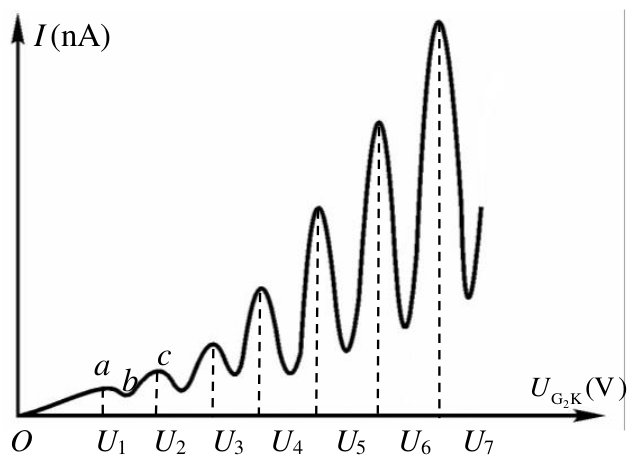
\includegraphics[scale=0.30]{p2.png}

由此可见,若 $eU_{G_{2}K}<\Delta{E}$则电子带着$eU_{G_{2}K}$的能
量进$G_{2}$-P区域。随着$U_{G_{2}K}$的增加,电流I增加(如图2中Oa段)。

当$eU_{G_{2}K}>=n\Delta{E}$时,电子与氩原子n次碰撞被吸收能量,板极电流I随加速电压$U_{G_{2}K}$变化曲线就形成n个峰值,如图2所示。相邻峰值之间的电压差$\Delta{U}$称为氩原子的第一激发电位。氩原子第一激发态与基态间的能级差为$$\Delta{E}=e\Delta{U}$$

\subsection{实验仪器}
微型弗兰克-赫兹实验仪(FD-FH-C,下面简称实验仪),示波器

\subsection{实验步骤}
\begin{enumerate}	
	\item[1)] 连接实验装置,按照实验仪的“出厂检验参考值”调整$U_{F}$、$U_{G_{1}K}$、$U_{G_{2}K]}$、$U_{G_{2}P}$,预热2min。后在参考值50\%范围分别调节上述4个电压参数,观察参数对激发电流的影响。
	\item[2)]
	将各参数调到参考值后,用实验仪的手动模式粗测出激发曲线的6个峰对应的$U_{G_{2}K}$。随后在10.0~95.0V内以0.5~2.0V为步长(在峰谷附近以0.5V为步长)改变$U_{G_{2}K}$,记录$I_{p}$数据。
\end{enumerate}

\section{实验现象及数据处理}
\subsection{调节$U_{F}$、$U_{G_{1}K}$、$U_{G_{2}K]}$、$U_{G_{2}P}$的实验现象和分析}
\subsubsection{现象}
\begin{enumerate}
	\item[$U_{F}$] 初始值为2.31V。$V_{F}$变大时,图像向纵向缓慢拉伸,手感类似于过阻尼振动,其中调节电压值类比于过阻尼振动中将弹簧的一端移动了一个位置。$V_{F}$变小时同理。
	\item[$U_{p}$] 初始值为9.39V。图像的纵向方向在一个$U_{p}$的平衡位置处最大(最宽),当$U_{p}$偏离平衡位置越大则图像越扁。且同时$U_{p}$变大时图像向上整体移动,$U_{p}$变小时整体向下移动。
	\item[$U_{G_{1}K}$] 初始值为1.30V。$U_{G_{1}K}$变大时,图像整体纵向拉伸。$U_{G_{1}K}$变小时,图像整体缩小。
	\item[$U_{G_{2}K}$] $U_{G_{2}K}$变大时扫描的范围变大,图像横坐标图像多出一部分。变小时同理。
\end{enumerate}

\subsubsection{分析}
\begin{enumerate}
	\item[$U_{F}$] $U_{F}$为灯丝的电压,$U_{F}$越高则灯丝的温度越高,发射的电子多故图像等比例的增大,且由于灯丝加热需要几秒钟的时间,所以调节$U_{F}$时图像会滞后与$U_{F}$的调节,创造出不跟手的手感。
	\item[$U_{p}$] $U_{p}$是最后的减速电压,用于筛选高于$U_{p}$能量的电子,故$U_{p}$越大,可以通过筛选的电子越小,电流也就越小,这解释了$U_{p}$增大时图像整体向下平移的现象。???
	\item[$U_{G_{1}K}$] $U_{G_{1}K}$为初始的加速电压,$U_{G_{1}K}$越大从灯丝飞出向$G_{1}$-$G_{2}$区间的电子数目增多,故图像随$U_{G_{1}K}$各部分近乎等比例的纵向拉伸。
	\item[$U_{G_{2}K}$] 由于在自动档下,$U_{G_{2}K}$仅仅对应扫描电压的平均值,故$U_{G_{2}K}$越大即扫描范围增大,故只是改变了图像的“定义域”。
\end{enumerate}

\subsection{氩原子激发曲线}
\subsubsection{数据处理方式}
先导入数据data,使用3次样条插值函数拟合数据。mathematica代码如下
\begin{lstlisting}[language=Mathematica]
fi = Interpolation[data, 
InterpolationOrder -> 3, 
Method -> "Spline"];
\end{lstlisting}

极小值点通过直接看表得出,如果有两个点都为极小值,则横坐标取这两点的平均值。本底电流的曲线会用3次样条函数拟合极小值坐标得到。下面放上拟合的代码。
\begin{lstlisting}[language=Mathematica]
lowfi = Interpolation[datalowpoints, 
InterpolationOrder -> 3, Method -> "Spline"]
\end{lstlisting}

画图时使用Plot函数,代码如下(其它画图参数省略)
\begin{lstlisting}[language=Mathematica]
Show[Plot[{fi[x], lowf[x], fi[x] - lowf[x]}, 
{x, 10, 95}], ListPlot[data]];
\end{lstlisting}
\subsubsection{图像以及分析}
下面是拟合的图像

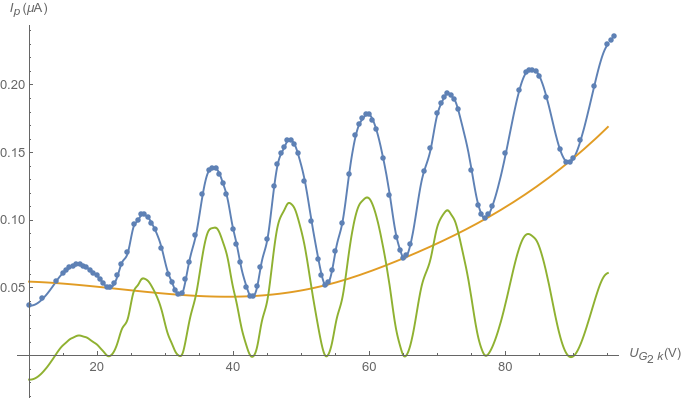
\includegraphics[scale=0.40]{data2.png}

以及自动模式下示波器画出来的图像

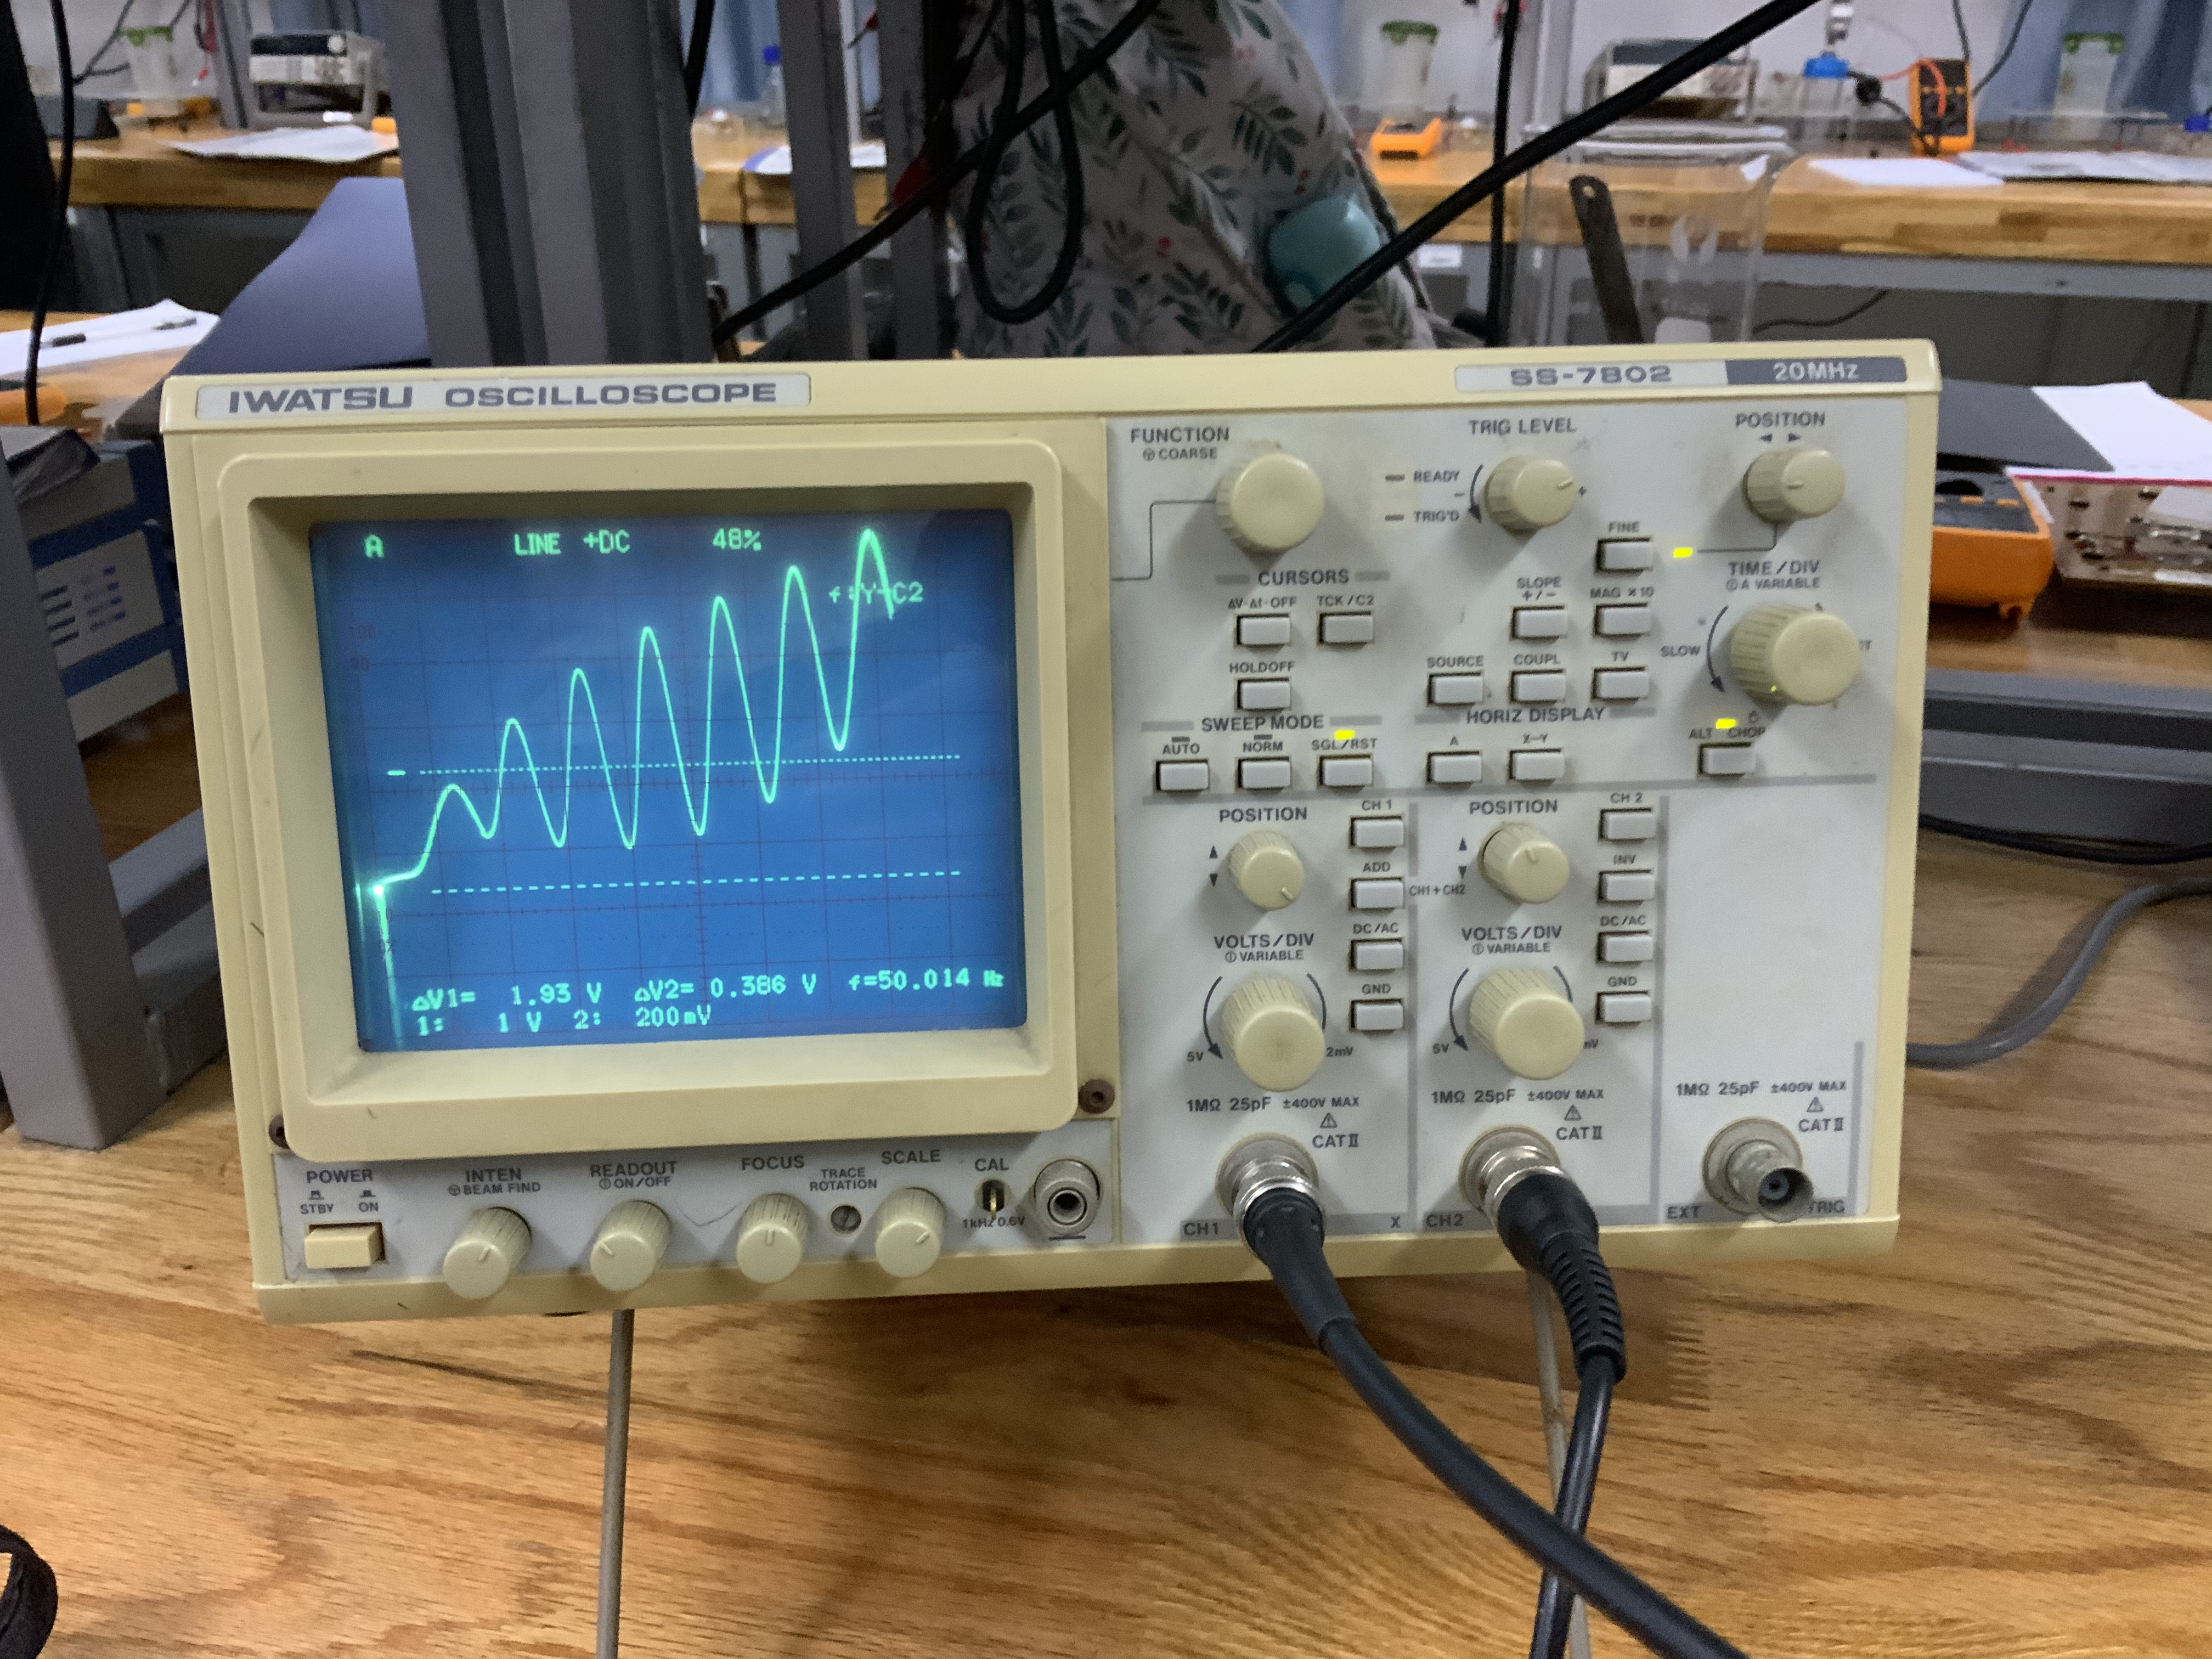
\includegraphics[scale=0.050]{p3.jpeg}

可以看出,拟合出的图像和实际上示波器显示的图像相差不大。

由极小值点的数据取平均得$$\Delta{U}=\dfrac{89.25-21.75}{6}V=10.75V$$
$$\Delta{E}=e\Delta{U}={1.602}\times{10^{-19}}C\times{10.75V}$$
$$=1.722\times10^{-18}J=10.75eV$$

百度上第一激发态到基态能级差为$1.63x10^{-18}J=10.17eV$(但百度上也有说是$11.8eV$的,前者根据跃迁释放122nm光子推导,后者是实验室测出的值)。

\subsection{汞蒸汽平均自由程计算}
已知在汞蒸气中电子的平均自由程$\lambda$与温度$T$、蒸气压$p$的关系为:
$$\lambda=\dfrac{kT}{\pi{r^2}p}$$
式中k为波尔兹曼常数,汞原子半径$r=0.176nm$。
在$80、90、100、160、170、180^\circ$时电子在汞蒸气的平均自由程分别为:
\begin{enumerate}
	\item[$80^\circ{C}$:] $\lambda=\dfrac{1.38\times10^{-23}\times(80+273.15)}{3.142\times(0.176\times10^{-9})^2\times{11.8}}=4.24mm$
	\item[$90^\circ{C}$:] $\lambda=\dfrac{1.38\times10^{-23}\times(90+273.15)}{3.142\times(0.176\times10^{-9})^2\times{21.1}}=2.44mm$
	\item[$100^\circ{C}$:] $\lambda=\dfrac{1.38\times10^{-23}\times(100+273.15)}{3.142\times(0.176\times10^{-9})^2\times{36.4}}=1.45mm$
	\item[$160^\circ{C}$:] $\lambda=\dfrac{1.38\times10^{-23}\times(160+273.15)}{3.142\times(0.176\times10^{-9})^2\times{558.5}}=0.109mm$
	\item[$170^\circ{C}$:] $\lambda=\dfrac{1.38\times10^{-23}\times(170+273.15)}{3.142\times(0.176\times10^{-9})^2\times{817.0}}=76.9\mu{m}$
	\item[$180^\circ{C}$:] $\lambda=\dfrac{1.38\times10^{-23}\times(180+273.15)}{3.142\times(0.176\times10^{-9})^2\times{1172.7}}=54.8\mu{m}$
\end{enumerate}

由此可见,当温度大于$160^\circ{C}$时,$\lambda<<d$(仪器尺寸),此时电子到达$G_{2}$时的动能基本都小于$\Delta{E}$,故此时$I_{p}$不太受温度影响。反而,当温度小于等于$100^\circ{C}$是,$\lambda$与d数量级相差不大,此时$I_{p}$受温度影响较大。

\subsection{实验总结}
此次实验测出氩的第一激发态与基态间能级相差10.75eV,且由$I_{p}$减去基底电流后大致关于$U_{G_{2}K}$成周期性变化支持了氩原子原子能级理论。

\subsection{思考题}
(1)$U_{G_{2}K}$\~{}$I_{p}$曲线电流下降并不十分陡峭,主要原因是什么?\\
答:如果没有碰撞则电子的速度服从电场下的玻耳兹曼分布(方差较大),就算$U_{G_{2}K}$刚好超过n倍的$I_{p}$,还是有相当部分电子动能小于n倍的$I_{p}$,所以下降并不是很陡峭。

(2)$I_{p}$的谷值并不为零,而且谷值依次沿$U_{G_{2}K}$轴升高,如何解释?\\
答:谷值不为0是因为和上道问题一样电子有分布,所以虽然平均值为$nI_{p}$,但是实际上动能偏离$nI_{p}$的电子导致谷值电流不为0。谷值沿$U_{G_{2}K}$轴升高可能一是因为$U_{G_{2}K}$增大时灯丝发射处于可以进入P板的动量方向的电子比例增大(不会被容器壁吸收或减速),所以$I_{p}$的谷值随这部分电子比例增加而升高。

(3)第一峰值所对应的电压是否等于第一激发电位?原因是什么?\\
答:不是严格等于。因为还是有波尔兹曼分布率的存在导致第一峰值激发电压与第一激发电位有所偏离。

(4)写出氩原子第一激发态与基态的能级差。\\
答:在上文中出现过了,由极小值点的数据取平均得$$\Delta{U}=\dfrac{89.25-21.75}{6}V=10.75V$$
$$\Delta{E}=e\Delta{U}={1.602}\times{10^{-19}}C\times{10.75V}$$
$$=1.722\times10^{-18}J=10.75eV$$

\subsection{参考文献}
\begin{enumerate}
	\item[[1]] 大学物理实验(第二册第二版),谢行怒、康士秀、霍剑青,高等教育出版社,2005.11,ISBN 7-04-017774-9
\end{enumerate}


\end{multicols}
\end{document}
